\chapter{Conclusion\label{cha:chapter7}}

 \begin{figure}[h]
 	\centering
 	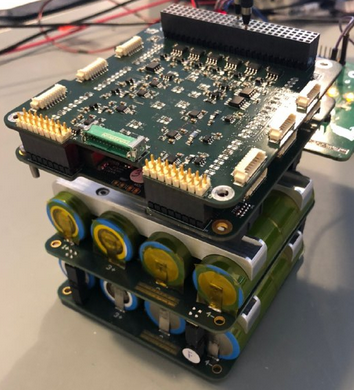
\includegraphics[scale=0.6]{EPS!.png}
 	\caption{EPS assembly (PPU, Battery board, PDU)}
 	\label{fig: EPS!}
 \end{figure}

This thesis has described development of the Power Distribution Unit that is designed in combination with Power Processing Unit and Battery case Unit to supply a Descartes satellite with a continuous orbital power.\\  


Massive work was made to accomplish all requirements and develop the PDU.

 One of the biggest challenge during the PDU design was the switches selection, and their placement on the PCB layout, taking into account the amount of components on the layout and the power channels requirements such as needed voltage, current, the trace width, size and ability to determine an over-current. Another big challenge was a layout structure of the PDU. Due the fact that PDU should not only be the distribution board for one Descartes mission, but universal distribution unit which might be adjusted for different upcoming missions without change of the design, but making little patch such as resistor replacement makes that master thesis arduous and interesting at the same time. Else, the PDU had some issues with a voltage drop on the Hispico line while initiation of S-band transceiver. The voltage drop occurred due to the high inrush current of the Hispico transceiver.    However, after the adding an extra capacitors on the output of the switch, voltage drop was reduced and results looked much more satisfied.    \\

PDU was tested individually by using microcontroller Nucleo STM32L073Rz with PSU as a power source and with a electrical load to simulate the load. 

After successful results, the PDU was tested using flight equipment such as PPU, which included a microcontroller to control the switches and receive data from current sensors, a battery board that provided power for the PDU, and payloads. 

Power Distribution Unit fits comfortably withing the mechanical structure of the 6U satellite, all the connectors are easily accessible. 
\\
The Power Distribution Board was designed by using Altium Designer and fabricated by Würth Electronics GmbH. All components were soldered by hands and tested according the test procedure, described in the Chapter \ref{6}. Most of the components were used in previous missions, which makes the PDU more promising for the upcoming mission.  \\

